Si bien es cierto que el $\mu$Arm, brazo en el que está basado el \pArm{}, 
ya es un sistema avanzado y capaz, como se explicó en la Introducción (\ref{ch:intro}),
el sistema desarrollado busca que pueda servir para ayudar y facilitar la entrada a
este tipo de tecnologías a otras personas, haciéndolo comprensible y, aprovechando
la tecnología de la impresión en 3D, fabricable por uno mismo.

Además, en relación a los \ac{ODS}, con el desarrollo de este sistema se pretende 
cumplir con los siguientes puntos:

\begin{itemize}
    \item [4 -] Educación de Calidad\footnote{\url{https://www.un.org/sustainabledevelopment/es/education/}}.
    \item [7 -] Energía Asequible y No Contaminante\footnote{\url{https://www.un.org/sustainabledevelopment/es/energy/}}.
    \item [10 -] Reducción de las desigualdades\footnote{\url{https://www.un.org/sustainabledevelopment/es/inequality/}}.
\end{itemize}

Para el primero, se tiene en cuenta que el producto se desarrolla siguiendo las 
iniciativas \ac{OS} y \ac{OH}, las cuales facilitan el acceso a la información a 
cualquiera que la requiera. %Además, se facilitará el desarrollo al completo, detallado y explicado, con la resolución de los problemas pertinentes y el porqué de ella.

Para el segundo, el \pArm{} usa la electricidad como fuente de energía, evitando
así otras más contaminantes como las producidas por combustibles fósiles. En añadido, 
se ha trabajado para que el consumo de energía sea el menor posible mediante el
estudio detallado del \ac{HW} que conforma la placa, permitiendo así un 
mayor tiempo de uso con la misma fuente de alimentación y no abusando de los recursos 
de los que se disponen.

Además, se ha buscado que el \pArm{} tenga un coste bajo, permitiendo así el 
acceso a los recursos y a los procesos de fabricación a todo el mundo que pudiera 
estar interesado. % y que disponga de la cantidad mínima necesaria para poder poner en funcionamiento el brazo robótico.

El apartado de la impresión 3D, como se ha visto anteriormente, puede suponer un
gran gasto a nivel tanto de recursos como de material debido a las impresiones
fallidas. Por suerte, el material fabricado por Ultimaker para sus impresoras
suele aprovechar materiales plásticos reciclados\footnote{\url{https://ultimaker.com/es/learn/100-recycled-filament-from-perpetual-plastic-project}}
y también existe una técnica que permite aprovechar las piezas fallidas y
generar nuevamente filamento que puede ser aprovechado para una nueva impresión.
Dicha técnica se conoce como ``\textit{filastruder}'', y el funcionamiento es
sencillo (más detalles en la imagen \ref{fig:filastruder}):

\begin{itemize}
    \item Se cogen las piezas inservibles y se ``trituran'' para hacerlas pequeñas.
    \item Se utiliza una cámara de calor para fundir el plástico.
    \item Mediante unas ruedas a presión, se extruye material renovado con el
    diámetro adecuado y se puede volver a utilizar para imprimir.
\end{itemize}

\begin{figure}[H]
    \centering
    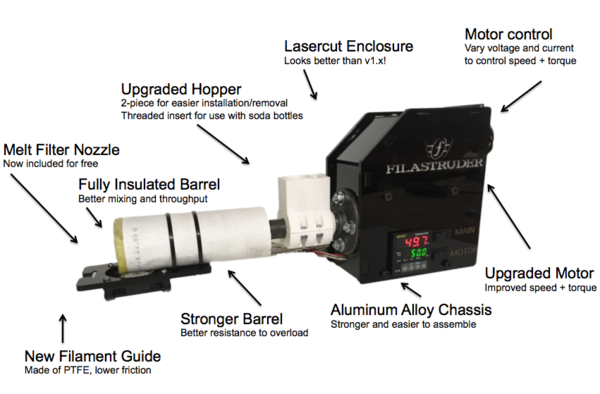
\includegraphics[width=.9\linewidth]{pictures/filastruder.png}
    \caption{Modo de funcionamiento del ``\textit{filastruder}'' \cite{filastruderFilastruderKit}.}
    \label{fig:filastruder}
\end{figure}

Durante el tiempo de desarrollo, no se contaban con estas herramientas, pero sería
perfectamente viable emplearlas para hacer un brazo robótico 100\% impreso con
materiales reciclados.